%
% wrpc_hdl.tex
%
% White Rabbit PTP Core HDL.
%

\documentclass[a4paper]{article}

\usepackage{fullpage}
\usepackage{graphicx}
\usepackage{multirow}
\usepackage{color}
\usepackage{colortbl}
\usepackage{array}
\usepackage{longtable}
\usepackage[latin1]{inputenc}
\usepackage{amsmath}
\usepackage{times,mathptmx}
\usepackage{chngcntr}
\usepackage{hyperref}

%%%%%%%%%%%%%%%%%%%%%%%%%%%%%%%%%%%%%%%%%%%%%%%%%%%%%%%%%%%%%%%%%%%%%%%%%%%
% creating subsubsubsection notation
% src: http://www.latex-community.org/forum/viewtopic.php?f=5&t=791
%%%%%%%%%%%%%%%%%%%%%%%%%%%%%%%%%%%%%%%%%%%%%%%%%%%%%%%%%%%%%%%%%%%%%%%%%%%
\setcounter{secnumdepth}{6}
\renewcommand\theparagraph{\Alph{paragraph}}

\makeatletter
\renewcommand\paragraph{\@startsection{paragraph}{4}{\z@}%
                                     {-3.25ex\@plus -1ex \@minus -.2ex}%
                                     {0.0001pt \@plus .2ex}%
                                     {\normalfont\normalsize\bfseries}}
\renewcommand\subparagraph{\@startsection{subparagraph}{5}{\z@}%
                                     {-3.25ex\@plus -1ex \@minus -.2ex}%
                                     {0.0001pt \@plus .2ex}%
                                     {\normalfont\normalsize\bfseries}}

%\renewcommand{\thefootnote}{\fnsymbol{footnote}}
%\renewcommand{\thefootnote}{\alph{footnote}}

\counterwithin{paragraph}{subsubsection}
\counterwithin{subparagraph}{paragraph}
\makeatother

%%%%%%%%%%%%%%%%%%%%%%%%%%%%%%%%%%%%%%%%%%%%%%%%%%%%%%%%%%%%%%%%%%%%%%%%%%%

\definecolor{wrlblue}{RGB}{165,195,210}
\definecolor{wrlgray}{RGB}{209,211,212}

\newcommand{\multirowpar}[2]{
  \multirow{#1}{\hsize}{\parbox{\hsize}{\strut\raggedright#2\strut}}
}

\newcommand{\hdltablesection}[1]{
  \multicolumn{4}{|c|}{\bf\small#1}
}

\newcolumntype{L}[1]{>{\raggedright\let\newline\\\arraybackslash\hspace{0pt}}m{#1}}
\newcolumntype{M}[1]{>{\raggedright\let\newline\\\arraybackslash\hspace{0pt}\ttsmall}m{#1}}
\newcolumntype{C}[1]{>{\centering\let\newline\\\arraybackslash\hspace{0pt}}m{#1}}
\newcolumntype{D}[1]{>{\centering\let\newline\\\arraybackslash\hspace{0pt}\ttsmall}m{#1}}
  
\newenvironment{hdlparamtable}{
  \let\underscore\_
  \renewcommand{\_}{\underscore\allowbreak}
  \setlength{\extrarowheight}{1pt}
  \begin{center}
    \begin{longtable}{|M{.2\textwidth}|C{.09\textwidth}|D{.11\textwidth}|L{.5\textwidth}|}
      \firsthline
      \rowcolor{wrlblue}
      \bf{name} & \bf{type} & \bf{default} & \bf{description}\\
      \hline
      \endhead
}{
  \lasthline
    \end{longtable}
  \end{center}
}

\newenvironment{hdlporttable}{
  \let\underscore\_
  \renewcommand{\_}{\underscore\allowbreak}
  \setlength{\extrarowheight}{1pt}
  \begin{center}
    \begin{longtable}{|M{.25\textwidth}|C{.05\textwidth}|D{.05\textwidth}|L{.55\textwidth}|}
      \firsthline
      \rowcolor{wrlblue}
      \bf{name} & \bf{dir} & \bf{size} & \bf{description}\\
      \hline
      \endhead
}{
  \lasthline
    \end{longtable}
  \end{center}
}

\def \wrpcrelease {for-tests}
%\def \wrpcrelease {wrpc-v4.0}

\newcommand{\tts}[1]{
  \texttt{\small{#1}}}

% same as \tts{}, without argument
\newcommand{\ttsmall}{\ttfamily\small}

\newcommand{\hrefwrpc}[1]{
  \tts{\href{http://www.ohwr.org/projects/wr-cores/repository/entry/#1?rev=\wrpcrelease}{#1}}}

\begin{document}

\title{White Rabbit PTP Core \\ HDL specification\\\normalsize
{version 1.0}\\\small{(01-03-2013)}}
\author{Grzegorz Daniluk\\ CERN BE-CO-HT}

\date{March 2017}
\maketitle
\thispagestyle{empty}

\newpage

\tableofcontents

\newpage

\section{Instantiating WRPC in your own HDL design}
\label{sec:wrpc_hdl}
This section describes the various options available to the users for instantiating and
parametrising the WRPC in their designs.

\begin{figure}[ht]
  \begin{center}
    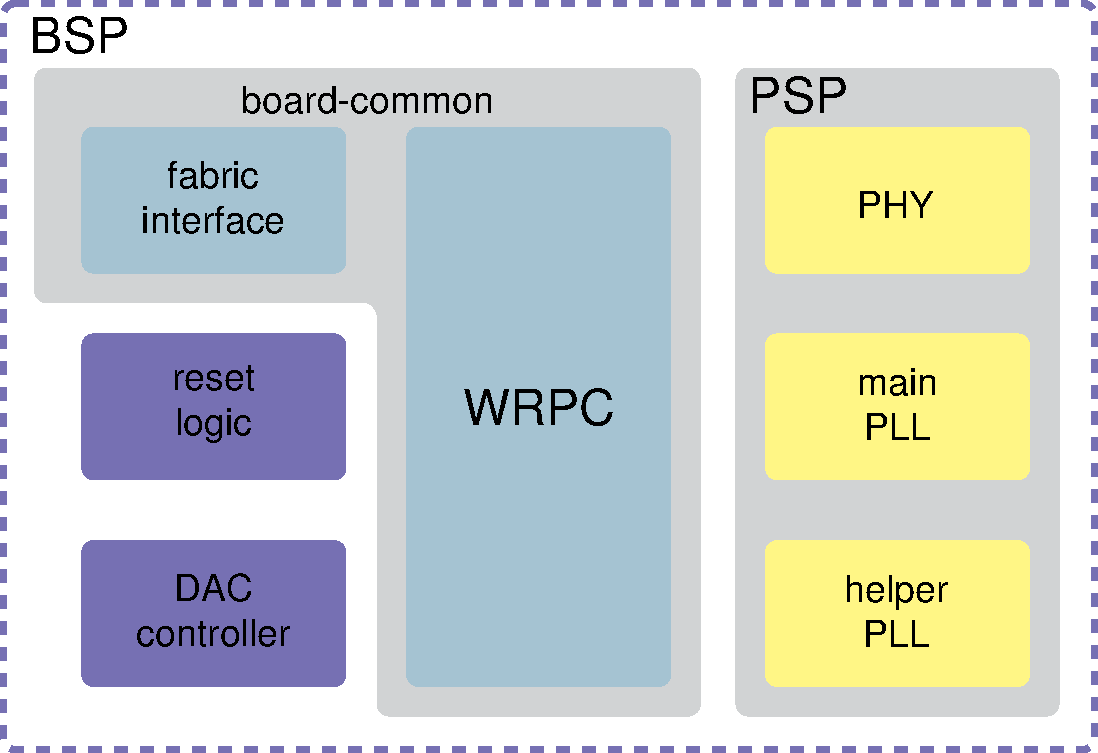
\includegraphics[width=.6\textwidth]{fig/wrpc_board.pdf}
    \caption{WRPC HDL abstraction hierarchy}
    \label{fig:wrpc_board}
  \end{center}
\end{figure}

The WRPC provides several levels of abstractions and VHDL modules, depending on the target
system. These are presented in Figure~\ref{fig:wrpc_board}. At the highest level of abstraction, the
WRPC provides Board Support Packages (BSPs), available for all officially supported boards. All BSP
modules share a common part (the ``board-common'' module) which encapsulates the WRPC core itself,
together with a selection of interfaces for connecting the core the the user FPGA
logic. Furthermore, each BSP also makes use of a Platform Support Package (PSP), which groups
together and instantiates all the FPGA-specific parts (typically hard IP provided by the FPGA
vendor), such as PHY, PLLs and clock buffers.

Thus, depending on the users' systems and needs, several scenarios might be available for
instantiating the WRPC into their designs.

\begin{description}
  \item[Option 1: Supported board.] In this simplest of scenarios, it will be enough to just
    instantiate the provided BSP into the users' designs and configure it via the provided generics.
  \item[Option 2: Supported FPGA platform.] The users could draw inspiration from an existing BSP
    based on the same platform, reusing the board-common module and PSP, while adapting the parts
    that are unique to their designs.
  \item[Option 3: Unsupported FPGA platform.] There is significant work involved in this
    scenario. In addition to providing the details for their board (just like for option 2), users
    also have to write their own PSP. It should be possible though to reuse the board-common
    module. Furthermore, if the unsupported platform is related to a supported one, it could be that
    the PHY and/or PLLs will also be reused, perhaps with minor adjustments.
\end{description}

When writing a new BSP or PSP, it's worth discussing it first in the
\href{http://www.ohwr.org/mailing_list/show?project_id=white-rabbit}{white-rabbit-dev} mailing
list. Perhaps there is already some preliminary support underway. It's also worth considering
sharing your work so that it can be merged with the project and added to the list of supported
platforms/boards.

The rest of this section describes the various modules in more detail. The WRPC module is presented
in Section~\ref{sec:hdl_wrpc}. The platform support modules are presented in
Section~\ref{sec:hdl_platform}, while the board support modules are presented in
Section~\ref{sec:hdl_board}.


\subsection{WR PTP Core component}
\label{sec:hdl_wrpc}
This section describes the input and output ports of the WRPC IP-core and VHDL generic parameters
that can be used to personalize the core.

The top-level VHDL module is located under:\\\hrefwrpc{modules/wrc\_core/wr\_core.vhd}

A wrapper for the top-level VHDL module which makes use of VHDL records to reduce the number of
ports can be found under:\\\hrefwrpc{modules/wrc\_core/xwr\_core.vhd}

\begin{figure}
  \begin{center}
    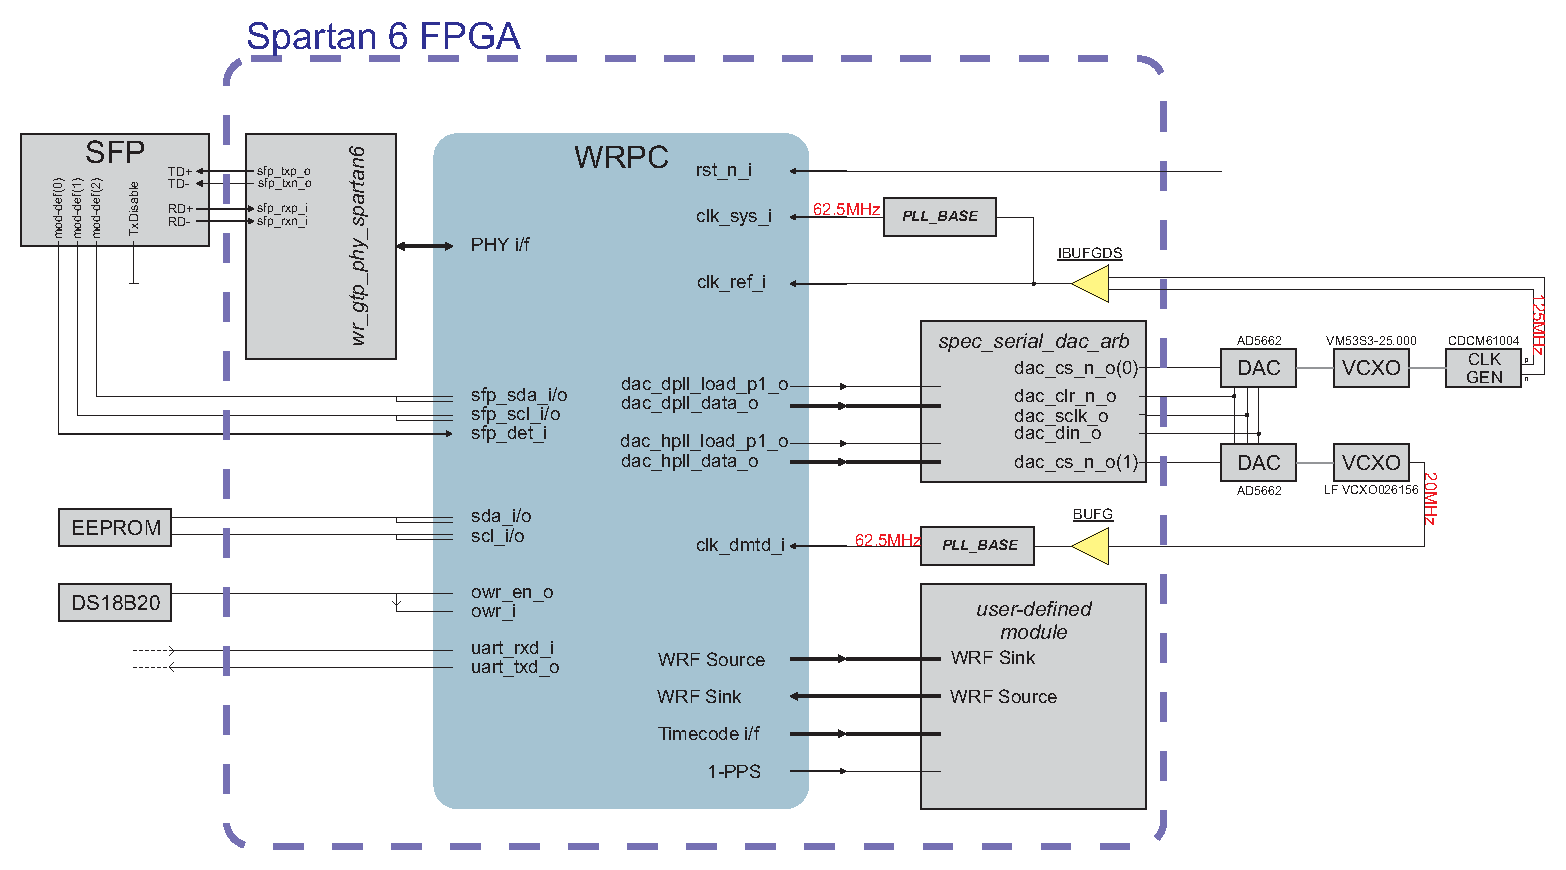
\includegraphics[width=.9\textheight, angle=270]{fig/basic_top.pdf}
    \caption{Simple top design with WRPC}
    \label{intro:fig:wrpc_top}
  \end{center}
\end{figure}

Figure \ref{intro:fig:wrpc_top} is an example on how to instantiate the WRPC component inside a
Xilinx Spartan6-based project. It contains few additional modules besides the WRPC:
\begin{itemize}
  \item \emph{wr\_gtp\_phy\_spartan6}: module wrapping Xilinx GTP SerDes to improve its determinism
  \item \emph{PLL\_BASE}: Xilinx Spartan6 PLL primitive\footnote{see also Xilinx Spartan-6 FPGA
    Clocking Resources, User Guide}, used to produce 62.5 MHz system clock from 125 MHz local
    reference clock and to produce the DMTD offset clock from a local 20 MHz oscillator
  \item \emph{spec\_serial\_dac\_arb}: converts DACs tuning values to serial interface and
    arbitrates access to two DACs used for reference and DMTD clock tuning.
\end{itemize}

A very similar example can be found in the WRPC reference design for PCI-Express SPEC board (see
Section~\ref{sec:hdl_board_spec}).


\subsubsection{Generic parameters}
\label{sec:wrc_generics}

\begin{hdlparamtable}
  g\_simulation & integer & 0 & setting to '1' speeds up the simulation,
  must be set to '0' for synthesis\\
  \hline
  g\_with\_external\_clock\_input & boolean & false &
  enable external clock and 1-PPS inputs. The PLL inside WRPC will lock to
  external 10 MHz and 1-PPS signal when operating in GrandMaster mode\\
  g\_phys\_uart & boolean & true & enable physical UART interface\\
  \hline
  g\_virtual\_uart & boolean & false & enable virtual UART interface\\
  \hline
  g\_aux\_clks & integer & 0 & number of aux clocks syntonized by WRPC to WR timebase\\
  \hline
  g\_rx\_buffer\_size & integer & 1024 & size of Rx buffer in WRPC MAC module,
  default value is 1024 and should not be changed\\
  \hline
  g\_tx\_runt\_padding & boolean & true & when set to true, all user frames
  transmitted from the external fabric interface are padded if shorter than
  minimal Ethernet frame size (60B with header)\\
  \hline
  g\_dpram\_initf & string & "" & filename of compiled WRPC software, to be
  stored in WRPC memory during the synthesis (default is \emph{wrc.ram}
  created by compiling WRPC software from \emph{wrpc-sw} git repository)\\
  \hline
  g\_dpram\_size & integer & 32768 & size of RAM used by WRPC software (in 32-bit
  words), default value is 22528 and should not be changed\\
  \hline
  g\_interface\_mode & enum& PIPELINED & external Wishbone Slave interface mode
  \tts{[PIPELINED/CLASSIC]}\\
  \hline
  g\_address\_granularity & enum & BYTE & granularity of address bus in external
  Wishbone Slave interface \tts{[BYTE/WORD]}\\
  \hline
  g\_aux\_sdb & rec & c\_wrc\_periph3\_sdb & structure providing an SDB descriptor
  for the peripheral attached to the WRPC auxiliary WB interface. This parameter is optional
  and can be left unassigned. The default value corresponds to an undocumented device with an
  address space of 256 bytes\\
  \hline
  g\_softpll\_enable\_debugger & boolean & false & when set to true, additional
  FIFO is instantiated in the SoftPLL for collecting DMTD tags. It can be read
  out by the host and analyzed for SoftPLL debugging.\\
  \hline
  g\_vuart\_fifo\_size & integer & 1024 & size (in bytes) for the virtual UART FIFO\\
  \hline
  g\_pcs\_16bit & boolean & false & when set to \tts{true}, make use of 16-bit PCS, otherwise use 8-bit PCS\\
  \hline
  g\_records\_for\_phy & boolean & false & when set to \tts{true}, all the PHY-related
  signals will be grouped in the \tts{phy8/phy16} VHDL records, otherwise the individual standard
  logic signals will be used\\
  \hline
  g\_diag\_id  & integer & 0 & auxiliary diagnostics module ID\\
  \hline
  g\_diag\_ver & integer  & 0 & auxiliary diagnostics version for a given module ID\\
  \hline
  g\_diag\_ro\_size & integer & 0 & number of read-only registers fed to auxiliary diagnostics\\
  \hline
  g\_diag\_rw\_size & integer & 0 & number of read-write registers fed to
  auxiliary diagnostics\\  
\end{hdlparamtable}

\subsubsection{Ports}
\label{sec:wrc_ports}

\begin{hdlporttable}
  \hdltablesection{Clocks and resets}\\
  \hline
  clk\_sys\_i & in & 1 & main system clock, can be any frequency $\leq f_{clk\_ref\_i}$
  e.g. 62.5~MHz\\
  \hline
  clk\_dmtd\_i & in & 1 & DMTD offset clock (close to 62.5 MHz, e.g. 62.49 MHz)\\
  \hline
  clk\_ref\_i & in & 1 & 125 MHz reference clock\\
  \hline
  clk\_aux\_i & in & var & [optional] vector of auxiliary
  clocks that will be disciplined to WR timebase. Size is equal to \tts{g\_aux\_clks}\\
  \hline
  clk\_ext\_mul\_i & in & 1 & 125 MHz clock, derived from \tts{clk\_ext\_i}\\
  \hline
  clk\_ext\_mul\_locked\_i & in & 1 & PLL locked indicator for \tts{clk\_ext\_mul\_i}\\
  \hline
  clk\_ext\_stopped\_i & in & 1 & PLL stopped indicator for \tts{clk\_ext\_mul\_i}\\
  \hline
  clk\_ext\_rst\_o & out & 1 & Reset output to be used for \tts{clk\_ext\_mul\_i}\\
  \hline  
  clk\_ext\_i & in & 1 & [optional] external 10 MHz reference clock input for
  GrandMaster mode\\
  \hline
  pps\_ext\_i & in & 1 & [optional] external 1-PPS input used in GrandMaster mode\\
  \hline
  rst\_n\_i & in & 1 & main reset input, active-low (hold for at least 5
  \tts{clk\_sys\_i} cycles)\\
  \hline\pagebreak
  \hdltablesection{Timing system}\\
  \hline
  dac\_hpll\_load\_p1\_o & out & 1 & validates DAC value on data port \\
  \hline
  dac\_hpll\_data\_o & out & 16 & DAC value for tuning helper (DMTD) VCXO\\
  \hline
  dac\_dpll\_load\_p1\_o & out & 1 & validates DAC value on data port \\
  \hline
  dac\_dpll\_data\_o & out & 16 & DAC value for tuning main (ref) VCXO\\
  \hline
  \hdltablesection{PHY inteface (when \tts{g\_records\_for\_phy = false})}\\
  \hline
  phy\_ref\_clk\_i & in & 1 & TX clock\\
  \hline
  phy\_tx\_data\_o & out & var & TX data. If \tts{g\_pcs\_16bit = true}, then \tts{size = 16}, else \tts{size=8}\\
  \hline
  phy\_tx\_k\_o & out & var & \tts{1} when \tts{phy\_tx\_data\_o} contains a control code, \tts{0} when it's a data byte. If \tts{g\_pcs\_16bit = true}, then \tts{size = 2}, else \tts{size=1}\\
  \hline
  phy\_tx\_disparity\_i & in  & 1 & disparity of the currently transmitted 8b10b code (\tts{1} for positive, \tts{0} for negative)\\
  \hline
  phy\_tx\_enc\_err\_i & in  & 1 & TX encoding error indication\\
  \hline
  phy\_rx\_data\_i & in & var & RX data. If \tts{g\_pcs\_16bit = true}, then \tts{size = 16}, else \tts{size=8}\\
  \hline
  phy\_rx\_rbclk\_i & in & 1 & RX recovered clock\\
  \hline
  phy\_rx\_k\_i & in & var & \tts{1} when \tts{phy\_rx\_data\_i} contains a control code, \tts{0} when it's a data byte. If \tts{g\_pcs\_16bit = true}, then \tts{size = 2}, else \tts{size=1}\\
  \hline
  phy\_rx\_enc\_err\_i & in & 1 & RX encoding error indication\\
  \hline
  phy\_rx\_bitslide\_i & in & var & RX bitslide indication. If \tts{g\_pcs\_16bit = true}, then \tts{size = 5}, else \tts{size=4}\\
  \hline
  phy\_rst\_o & out & 1 & PHY reset, active high\\
  \hline
  phy\_rdy\_i & in & 1 & PHY is ready: locked and aligned\\
  \hline
  phy\_loopen\_o & out & 1 & \multirowpar{2}{local loopback enable (TX$\rightarrow$RX), active high}\\
  \cline{1-3}
  phy\_loopen\_vec\_o & out & 3 &\\
  \hline
  phy\_tx\_prbs\_sel\_o & out & 3 & PRBS select (see Xilinx UG386 Table 3-15; "000" = Standard operation, pattern generator off)\\
  \hline
  phy\_sfp\_tx\_fault\_i & in & 1 & SFP TX fault indicator\\
  \hline
  phy\_sfp\_los\_i & in & 1 & SFP Loss Of Signal indicator\\
  \hline
  phy\_sfp\_tx\_disable\_o & out & 1 & SFP TX disable control\\
  \hline
  \hdltablesection{PHY inteface (when \tts{g\_records\_for\_phy = true})}\\
  \hline
  phy8\_o & out & rec & \multirowpar{2}{input/output records for PHY signals
    when \tts{g\_pcs\_16bit = false}}\\
  \cline{1-3}
  phy8\_i & in & rec & \\
  \hline
  phy16\_o & out & rec & \multirowpar{2}{input/output records for PHY signals
    when \tts{g\_pcs\_16bit = true}}\\
  \cline{1-3}
  phy16\_i & in & rec & \\
  \hline\pagebreak
  \hdltablesection{GPIO}\\
  \hline
  led\_act\_o & out & 1 & signal for driving Ethernet activity LED\\
  \hline
  led\_link\_o & out & 1 & signal for driving Ethernet link LED\\
  \hline
  sda\_i & in  & 1 & \multirowpar{4}{I2C interface for EEPROM memory storing calibration}\\
  \cline{1-3}
  sda\_o & out & 1 & \\
  \cline{1-3}
  scl\_i & in  & 1 & \\
  \cline{1-3}
  scl\_o & out & 1 & \\
  \hline
  sfp\_sda\_i & in  & 1 & \multirowpar{4}{I2C interface for EEPROM inside SFP module}\\
  \cline{1-3}
  sfp\_sda\_o & out & 1 & \\
  \cline{1-3}
  sfp\_scl\_i & in  & 1 & \\
  \cline{1-3}
  sfp\_scl\_o & out & 1 & \\
  \hline
  sfp\_det\_i & in & 1 & SFP presence indicator\\
  \hline
  btn1\_i & in & 1 & \multirowpar{2}{two microswitch inputs, active low, currently not
    used in official WRPC software}\\
  \cline{1-3}
  btn2\_i & in & 1 & \\
  \hline
  spi\_sclk\_o & out & 1 & Flash SPI SCLK\\
  \hline
  spi\_ncs\_o  & out & 1 & Flash SPI $\overline{\mbox{SS}}$\\
  \hline
  spi\_mosi\_o & out & 1 & Flash SPI MOSI\\
  \hline
  spi\_miso\_i & in  & 1 & Flash SPI MISO\\
  \hline
  \hdltablesection{UART}\\
  \hline
  uart\_rxd\_i & in  & 1 & \multirowpar{2}{[optional] serial UART interface for
    interaction with WRPC software}\\
  \cline{1-3}
  uart\_txd\_o & out & 1 & \\
  \hline
  \hdltablesection{OneWire}\\
  \hline
  owr\_pwren\_o & out & 1 & \multirowpar{3}{[optional] 1-Wire interface used to read the
    temperature of hardware board from digital thermometer (e.g. Dallas DS18B20)}\\
  \cline{1-3}
  owr\_en\_o & out & 1 & \\
  \cline{1-3}
  owr\_i & in & 1 & \\
  \hline
  \hdltablesection{External WB interface}\\
  \hline
  wb\_adr\_i   & in & 32 & \multirowpar{11}{Wishbone slave interface that operates in
    Pipelined or Classic mode (selected with \tts{g\_interface\_mode}), with the address
    bus granularity controlled with \tts{g\_address\_granularity}}\\
  \cline{1-3}
  wb\_dat\_i   & in & 32 &\\
  \cline{1-3}
  wb\_dat\_o   & out & 32 &\\
  \cline{1-3}
  wb\_sel\_i   & in & 4 & \\
  \cline{1-3}
  wb\_we\_i    & in & 1 & \\
  \cline{1-3}
  wb\_cyc\_i   & in & 1 & \\
  \cline{1-3}
  wb\_stb\_i   & in & 1 & \\
  \cline{1-3}
  wb\_ack\_o   & out & 1 & \\
  \cline{1-3}
  wb\_err\_o   & out & 1 & \\
  \cline{1-3}
  wb\_rty\_o   & out & 1 & \\
  \cline{1-3}
  wb\_stall\_o & out & 1 & \\
  \hline
  wb\_slave\_o & out & rec & \multirowpar{2}{Alternative record-based ports
    for the WB slave interface (available in \tts{xwr\_core.vhd})}\\
  \cline{1-3}
  wb\_slave\_i & in & rec & \\
  \hline\pagebreak
  \hdltablesection{Auxiliary WB master}\\
  \hline
  aux\_adr\_i   & in & 32 & \multirowpar{11}{Auxilirary Wishbone pipelined
    master interface}\\
  \cline{1-3}
  aux\_dat\_o   & out & 32 &\\
  \cline{1-3}
  aux\_dat\_i   & in  & 32 &\\
  \cline{1-3}
  aux\_sel\_o   & out & 4 & \\
  \cline{1-3}
  aux\_we\_o    & out & 1 & \\
  \cline{1-3}
  aux\_cyc\_o   & out & 1 & \\
  \cline{1-3}
  aux\_stb\_o   & out & 1 & \\
  \cline{1-3}
  aux\_ack\_i   & in  & 1 & \\
  \cline{1-3}
  aux\_stall\_i & in  & 1 & \\
  \hline
  aux\_master\_o & out & rec & \multirowpar{2}{Alternative record-based
    ports for the aux WB master interface (available in \tts{xwr\_core.vhd})}\\
  \cline{1-3}
  aux\_master\_i & in & rec & \\
  \hline
  \hdltablesection{External fabric interface}\\
  \hline
  ext\_snk\_adr\_i & in & 2 & \multirowpar{9}{External fabric Wishbone
    pipelined interface, direction Sink$\rightarrow$Source}\\
  \cline{1-3}
  ext\_snk\_dat\_i & in & 16 & \\
  \cline{1-3}
  ext\_snk\_sel\_i & in & 2 & \\
  \cline{1-3}
  ext\_snk\_cyc\_i & in & 1 & \\
  \cline{1-3}
  ext\_snk\_stb\_i & in & 1 & \\
  \cline{1-3}
  ext\_snk\_we\_i  & in & 1 & \\
  \cline{1-3}
  ext\_snk\_ack\_o & out & 1 & \\
  \cline{1-3}
  ext\_snk\_err\_o & out & 1 & \\
  \cline{1-3}
  ext\_snk\_stall\_o & out & 1 & \\
  \hline
  ext\_src\_adr\_o & out & 2 & \multirowpar{9}{External fabric Wishbone
    pipelined interface, direction Source$\rightarrow$Sink}\\
  \cline{1-3}
  ext\_src\_dat\_o & out & 16 & \\
  \cline{1-3}
  ext\_src\_sel\_o & out & 2 & \\
  \cline{1-3}
  ext\_src\_cyc\_o & out & 1 & \\
  \cline{1-3}
  ext\_src\_stb\_o & out & 1 & \\
  \cline{1-3}
  ext\_src\_we\_o  & out & 1 & \\
  \cline{1-3}
  ext\_src\_ack\_i & in & 1 & \\
  \cline{1-3}
  ext\_src\_err\_i & in & 1 & \\
  \cline{1-3}
  ext\_src\_stall\_i & in & 1 & \\
  \hline
  wrf\_src\_o & out & rec & \multirowpar{4}{Alternative record-based
    ports for the fabric interface (available in \tts{xwr\_core.vhd})}\\
  \cline{1-3}
  wrf\_src\_i & in &  rec & \\
  \cline{1-3}
  wrf\_snk\_o & out & rec & \\
  \cline{1-3}
  wrf\_snk\_i & in &  rec & \\
  \hline\pagebreak
  \hdltablesection{External TX timestamp interface}\\
  \hline
  txtsu\_port\_id\_o & out & 5 & physical port ID from which the timestamp
  was originated. WRPC has only one physical port, so this value is always
  \tts{0}.\\
  \hline
  txtsu\_frame\_id\_o & out & 16 & frame ID for which the timestamp is
  available\\
  \hline
  txtsu\_ts\_value\_o & out & 32 & Tx timestamp value\\
  \hline
  txtsu\_ts\_incorrect\_o & out & 1 & Tx timestamp is not reliable since it
  was generated while PPS generator inside WRPC was being adjusted\\
  \hline
  txtsu\_stb\_o & out & 1 & strobe signal that validates the rest of signals
  described above\\
  \hline
  timestamps\_o & out & rec & Alternative record-based output ports for
  the TX timestamp interface (available in \tts{xwr\_core.vhd})\\
  \hline
  txtsu\_ack\_i & in & 1 & acknowledge, indicating that user-defined module
  has received the timestamp\\
  \hline
  \hdltablesection{Pause frame control}\\
  \hline
  fc\_tx\_pause\_req\_i   & in  &  1 & Ethernet flow control, request sending
  Pause frame\\
  \hline
  fc\_tx\_pause\_delay\_i & in  & 16 & Pause quanta\\
  \hline
  fc\_tx\_pause\_ready\_o & out &  1 & Pause acknowledge - active after the
  current pause send request has been completed\\
  \hline
  \hdltablesection{Timecode/Servo control}\\
  \hline
  tm\_link\_up\_o & out & 1 & state of Ethernet link (up/down), \tts{1}
  means Ethernet link is up\\
  \hline
  tm\_dac\_value\_o & out & 24 & DAC value for tuning auxiliary clock
  (\tts{clk\_aux\_i})\\
  \hline
  tm\_dac\_wr\_o & out & var & validates auxiliary DAC value. Size is equal
  to \tts{g\_aux\_clks}\\
  \hline
  tm\_clk\_aux\_lock\_en\_i & in & var & enable locking auxiliary clock to
  internal WR clock. Size is equal to \tts{g\_aux\_clks}\\
  \hline
  tm\_clk\_aux\_locked\_o & out & var & auxiliary clock locked to internal WR
  clock. Size is equal to \tts{g\_aux\_clks}\\
  \hline
  tm\_time\_valid\_o & out & 1 & if \tts{1}, the timecode generated by the
  WRPC is valid\\
  \hline
  tm\_tai\_o & out & 40 & TAI part of the timecode (full seconds)\\
  \hline
  tm\_cycles\_o & out & 28 & fractional part of each second represented by
  the state of counter clocked with the frequency 125 MHz (values from 0 to
  124999999, each count is 8 ns)\\
  \hline
  pps\_p\_o & out & 1 & 1-PPS signal generated in \tts{clk\_ref\_i} clock
  domain and aligned to WR time, pulse generated when the cycle counter is 0
  (beginning of each full TAI second)\\
  \hline
  pps\_led\_o & out & 1 & 1-PPS signal with extended pulse width to drive a LED\\
  \hline
  rst\_aux\_n\_o & out & 1 & Auxiliary reset output, active low\\  
  \hline
  link\_ok\_o & out & 1 & Link status indicator\\
  \hline
  \hdltablesection{Auxiliary diagnostics to/from external modules}\\
  \hline
  \linebreak aux\_diag\_i\linebreak & in & var & \multirowpar{2}{Arrays of
    32-bit vectors, to be accessed from WRPC via SNMP or uart console. Input array
    contains \tts{g\_diag\_ro\_size} elements, while output array contains
    \tts{g\_diag\_rw\_size} elements}\\
  \cline{1-3}
  \linebreak aux\_diag\_o\linebreak & out & var & \\
\end{hdlporttable}

\subsection{PHY interface}

\begin{figure}[ht]
  \begin{center}
    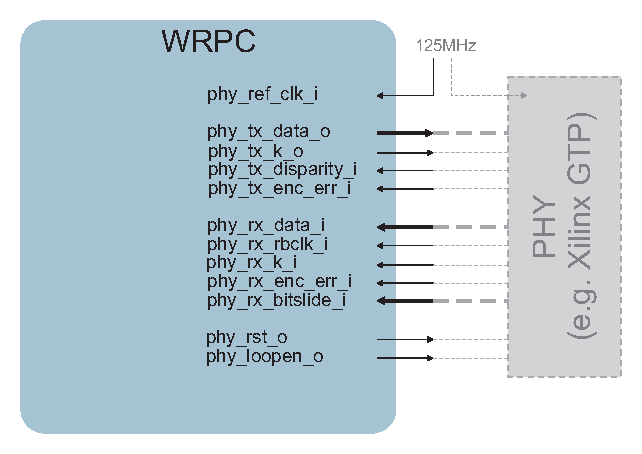
\includegraphics[width=.7\textwidth]{fig/wrpc_phyif.pdf}
    \caption{PHY interface of WRPC}
  \end{center}
\end{figure}

The interface connects WRPC with the Ethernet PHY layer IP-core. The interface is
generic, but currently two Gigabit Ethernet PHYs are tested and supported: Xilinx
8-bit GTP and 16-bit GTX SerDes. The signals' naming convention is the same as
in the GTP/GTX component definition.\\

{\bf Important !} If a WRPC user wants to use one of the supported PHYs (GTP,
GTX), they have to be taken from the White Rabbit HDL package instead of generating
them with the Xilinx Coregen tool. That is because WR developers have attached
additional logic to Xilinx GTP/GTX to improve its determinism.\\

\subsection{GPIO/UART/I2C/1-Wire/SPI interfaces}
\label{sec:wrpc_periph}

%\begin{figure}[ht]
%  \begin{center}
%    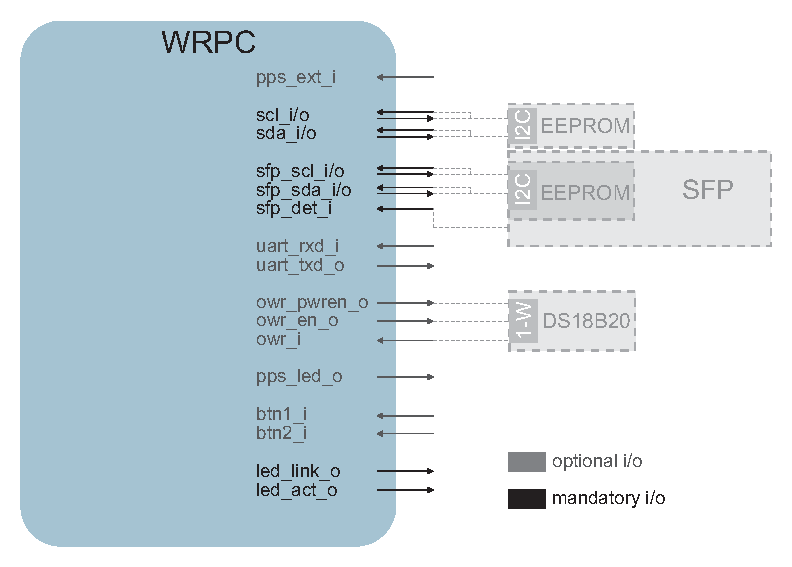
\includegraphics[width=.9\textwidth]{fig/basic_wrpc_gpio.pdf}
%    \caption{Other interfaces of WRPC}
%  \end{center}
%\end{figure}

Several hardware peripherals can be connected to the White Rabbit PTP Core. It
has:
\begin{itemize}
  \item UART - provides access to the WR PTP Core user shell
  \item 1-Wire - access to a digital thermometer for an on-board temperature and
    unique ID (used to generate a default MAC address of the WR port)
  \item SFP $I^2C$ - access to the SFP EEPROM, to read its ID and math with the
    calibration values
  \item SPI - access to the Flash memory, used to store calibration
    parameters and init script
  \item EEPROM $I^2C$ - [optional] access to the EEPROM memory, used to store
    calibration parameters and init script - currently SPI Flash is the
    preferred storage, however, EEPROM can still be used if needed.
\end{itemize}

\subsection{External Wishbone Slave/Master interface}

\begin{figure}[ht]
  \begin{center}
    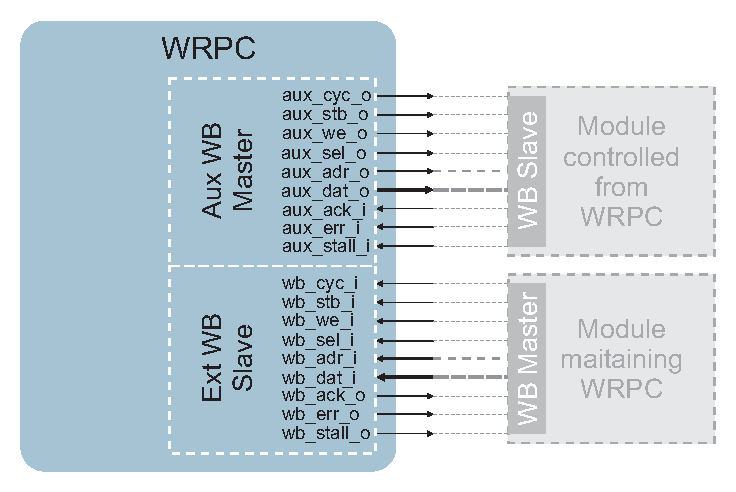
\includegraphics[width=.7\textwidth]{fig/wrpc_wb.pdf}
    \caption{External Wishbone interfaces of WRPC}
  \end{center}
\end{figure}

{\bf Aux WB Master} is a Pipelined Wishbone Master interface. It is connected
through the Wishbone Crossbar inside the White Rabbit PTP Core to the LM32 soft-core
processor (instantiated inside the WRPC). It can optionally be used to control
any user-defined module having a Pipelined Wishbone Slave interface. In that case, the WRPC software
has to be modified to control additional modules connected to the \emph{Aux WB
Master} interface.\\

{\bf Ext WB Slave} is a Wishbone Slave interface that operates in Pipelined or
Classic mode (selected with \emph{g\_interface\_mode} generic), with the address bus
granularity set with \linebreak \emph{g\_address\_granularity} generic. It gives the access
to control all the WRPC internals. In the WRPC reference design it is connected to
the Gennum GN4124 IP-core and used to upload WRPC software to its internal memory.\\

HDL modules accessible through \emph{Ext WB Slave} interface:
\begin{center}
  \begin{tabular}{|l|l|}
    \hline {\bf module name} & {\bf offset (bytes)}\\
    \hline
    WRPC internal memory & 0x00000\\
                Mini NIC & 0x20000\\
                Endpoint & 0x20100\\
                Soft PLL & 0x20200\\
           PPS generator & 0x20300\\
                  Syscon & 0x20400\\
                    UART & 0x20500\\
           1-Wire Master & 0x20600\\
           Aux WB Master & 0x20700\\
    \hline
  \end{tabular}
\end{center}

\subsubsection{Fabric interface}
\label{sec:wrpc_fabric}

The Fabric interface is used for sending and receiving Ethernet frames. It consists 
of two pipelined Wishbone interfaces operating independently: 

\begin{itemize}
  \item \emph{WRF Source}: pipelined Wishbone Master, passes all the Ethernet frames
    received from a physical link to WRF Sink interface implemented in a
    user-defined module.
  \item \emph{WRF Sink}: pipelined Wishbone Slave, receives Ethernet frames from
    the WRF Source implemented in the user-defined module, and sends them to a
    physical link.
\end{itemize}

{\bf Address bus} can have one of the following values:

\begin{center}
\begin{tabular}{|c|l|}
  \hline {\bf decimal value} & {\bf meaning of data word on data bus}\\
  \hline
  \emph{0} & regular data (packet header and payload)\\
  \emph{1} & OOB (Out-of-band) data\\
  \emph{2} & status word\\
  \emph{3} & currently not used\\
  \hline
\end{tabular}
\end{center}

{\bf Status word} (sent when the value of address bus is \emph{2}) contains
various information about Ethernet frame's structure and type:
%\begin{figure}[ht]
  \begin{center}
    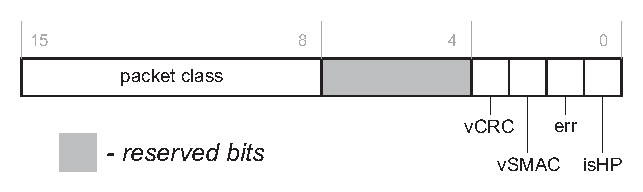
\includegraphics[width=.6\textwidth]{fig/status.pdf}
    %\caption{Status word format}
  \end{center}
%\end{figure}

\begin{itemize}
  \item[] \emph{isHP} - if \emph{1}, the frame is high priority
  \item[] \emph{err} - if \emph{1}, the frame contains an error
  \item[] \emph{vSMAC} - the frame contains a source MAC address (otherwise
    it will be assigned from WRPC configuration)
  \item[] \emph{vCRC} - the frame contains a valid CRC checksum
  \item[] \emph{packet class} - the packet class assigned by the classifier
    inside WRPC MAC module
\end{itemize}

OOB data is used for passing the timestamp-related information for the incoming and 
outgoing Ethernet frames. Each frame received from a physical link is
timestamped inside the WRPC and this value is passed as Rx OOB
data. On the other hand, for each transmitted frame the Tx timestamp can be read
from the Tx Timestamping Interface (section \ref{sec:txts}) together with a unique
frame number assigned in Tx OOB. Therefore, the format of OOB differs between Rx
and Tx frames.\\

{\bf Tx OOB format}:

%\begin{figure}[ht]
  \begin{center}
    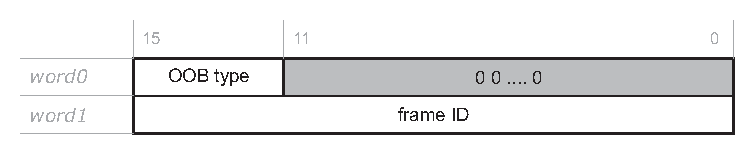
\includegraphics[width=.7\textwidth]{fig/oob_tx.pdf}
    %\caption{Tx OOB data format}
    %\label{fig:fabric_adv:tx_oob}
  \end{center}
%\end{figure}

\begin{itemize}
  \item[] \emph{OOB type}: "0001" means Tx OOB
  \item[] \emph{frame ID}: ID of the frame being sent. It is later output
    through the \emph{Tx Timestamping interface} to associate Tx timestamp with
    appropriate frame. Frame ID = 0 is reserved for PTP packets inside WRPC
    and cannot be used by user-defined modules.
\end{itemize}

{\bf Rx OOB format}:
%\begin{figure}[ht]
  \begin{center}
    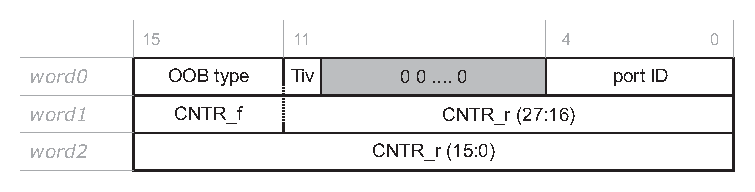
\includegraphics[width=.7\textwidth]{fig/oob_rx.pdf}
    %\caption{Rx OOB data format}
    %\label{fig:fabric_adv:rx_oob}
  \end{center}
%\end{figure}

\begin{itemize}
  \item[] \emph{OOB type}: "0000" means Rx OOB
  \item[] \emph{Tiv}: timestamp invalid. When this bit is set to '1', the PPS
    generator inside WRPC is being adjusted which means the Rx timestamp is not
    reliable.
  \item[] \emph{port ID}: the ID of a physical port on which the packet was
    received. In case of WRPC, this field is always 0, because there is only one
    physical port available.
  \item[] \emph{CNTR\_f}: least significant bits of the Rx timestamp generated on
    the falling edge of the reference clock.
  \item[] \emph{CNTR\_r}: Rx timestamp generated on the rising edge of the reference
    clock.
\end{itemize}

\begin{figure}
  \begin{center}
    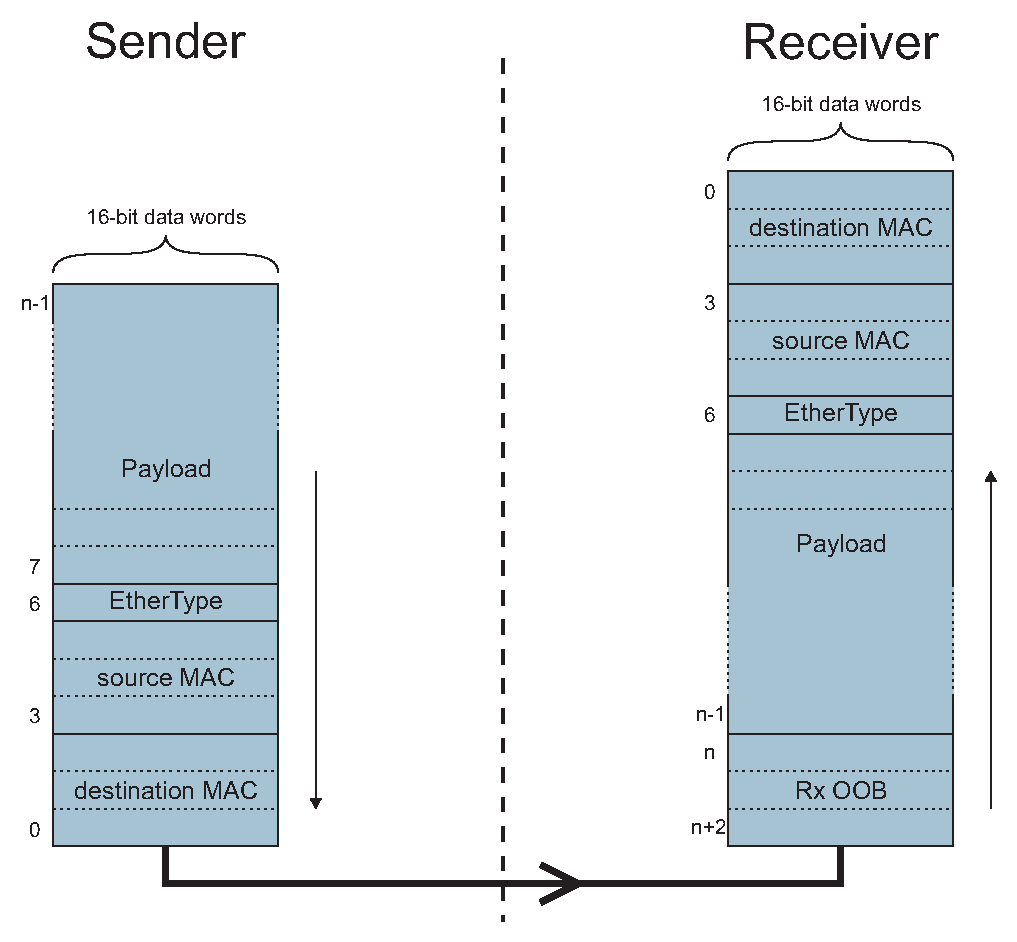
\includegraphics[width=.6\textwidth]{fig/basic_wrf_data.pdf}
    \caption{Data words that make the Ethernet frame}
    \label{fig:fabric:simple_data}
  \end{center}
\end{figure}

Figure \ref{fig:fabric:simple_data} presents data words fed to the WRF
data bus by the sender and the information got at the receiving side. Please
note that the CRC checksum is calculated and inserted automatically inside the
WRPC and user-defined module doesn't care about it. The Ethernet frame received
from the WR Fabric interface may contain additional OOB data suffixed. It has to
be received (acknowledged) by the user-defined module, but can be simply discarded.

\newparagraph{Examples}
Figure \ref{fig:fabric:simple_tx} shows a very simple WR Fabric cycle. The WRF
Source of user-defined module sends there an Ethernet frame containing even
number of bytes.

\begin{figure}
  \begin{center}
    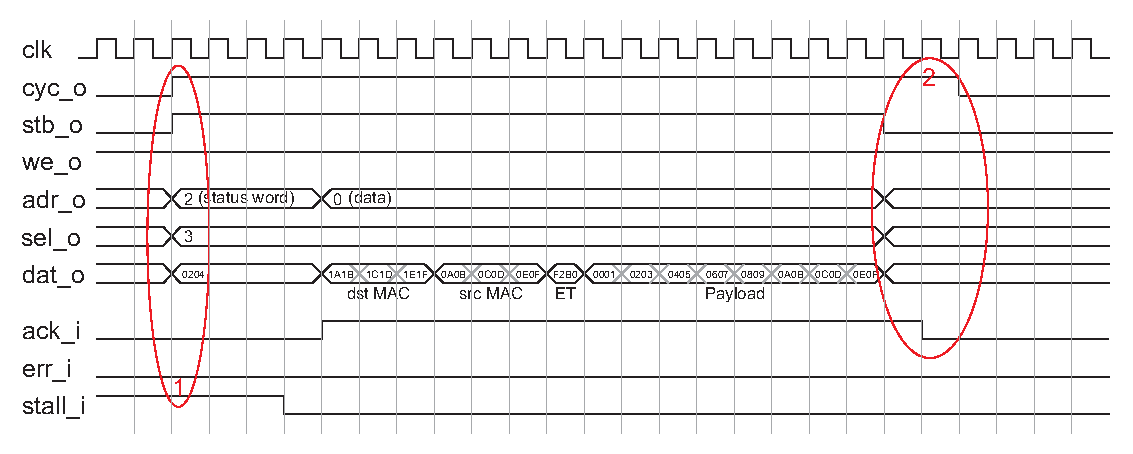
\includegraphics[width=\textwidth]{fig/basic_wrf_cycle_simple.pdf}
    \caption{Simple WR Fabric cycle - user-defined module sending packet}
    \label{fig:fabric:simple_tx}
  \end{center}
\end{figure}

\begin{enumerate}
  \item The WRF Source in user-defined module starts the cycle by asserting
    \emph{cyc\_o}, \emph{stb\_o} and putting a status word to the data bus.
    However, since WRF Sink set \emph{stall} signal to active state, Source has
    to wait until Sink is ready to receive data.
  \item After the last word is transmitted, the WRF Source sets \emph{stb\_o} back
    to \emph{0}, but waits until Sink acknowledges all the words transmitted in
    the cycle (\emph{ack\_i} line). The cycle ends when \emph{cyc\_o} goes back
    to the low state.
\end{enumerate}

Figure \ref{fig:fabric:sel} shows again a very simple WR Fabric cycle where
user-defined WRF Source sends an Ethernet frame to the WRPC. This time though,
the frame contains odd number of bytes, therefore the \emph{sel} line is used to
signal this fact to WRF Sink inside the WRPC (1).

\begin{figure}
  \begin{center}
    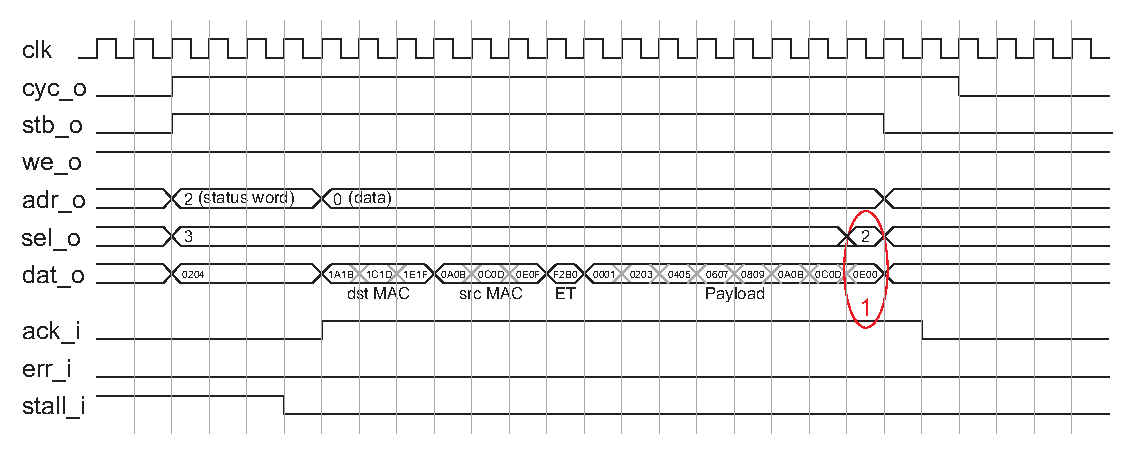
\includegraphics[width=\textwidth]{fig/basic_wrf_cycle_sel.pdf}
    \caption{Simple WR Fabric cycle - user-defined module sending packet(odd
    number of bytes in the payload)}
    \label{fig:fabric:sel}
  \end{center}
\end{figure}

Figure \ref{fig:fabric:cyc} presents more complicated Fabric cycle where an
Ethernet frame is received from WRF Source in the WRPC (output signals in the
diagram are driven by WRF Source on the WRPC side): 

\begin{figure}
  \begin{center}
    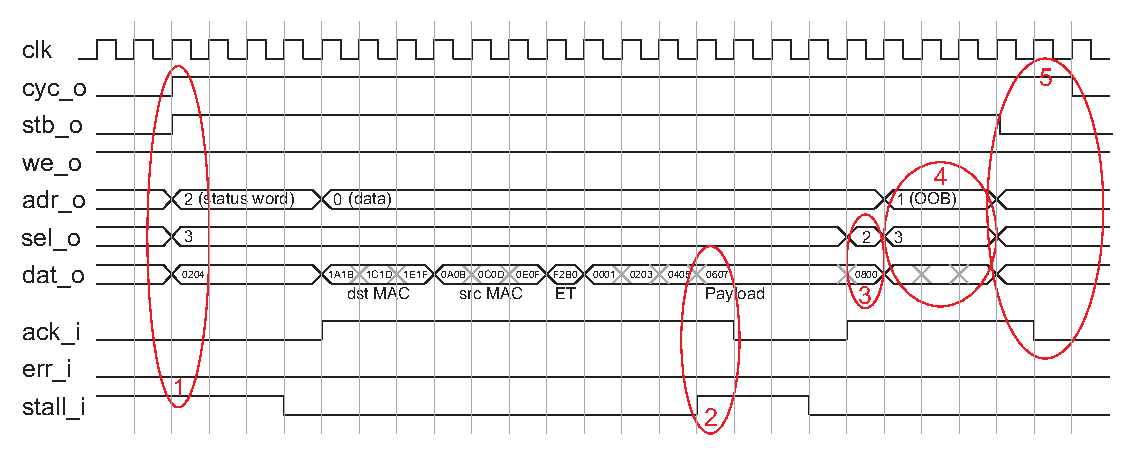
\includegraphics[width=\textwidth]{fig/basic_wrf_cycle.pdf}
    \caption{WR Fabric cycle}
    \label{fig:fabric:cyc}
  \end{center}
\end{figure}
\begin{enumerate}
  \item The WRF Source starts the cycle by asserting \emph{cyc\_o}, \emph{stb\_o}
    and putting a status word to the data bus. However, since WRF Sink set 
    \emph{stall} signal to active state, Source has to wait until Sink is ready
    to receive data.
  \item While the payload of the Ethernet frame is being transmitted, Sink
    stalls the cycle. The WRF Source pauses the transmission until Sink becomes
    ready to process the rest of the data. During that time \emph{stb\_o} has to
    remain in a high state.
  \item The Ethernet frame contains an odd number of bytes, so only half of last
    word of payload carries a valid data. \emph{Sel\_o} is used to signal this
    fact to WRF Sink.
  \item After the whole payload is transmitted, Source may additionally sent Rx
    OOB data. It contains some internal WRPC data that should be acknowledged
    by Sink, but discarded in the user's module.
  \item After the last word is transmitted, the WRF Source sets \emph{stb\_o} back
    to \emph{0}, but waits until Sink acknowledges all the words transmitted in
    the cycle (\emph{ack\_i} line). The cycle ends when \emph{cyc\_o} goes back
    to the low state.
\end{enumerate}

WRF Sink can use the \emph{stall} line to pause the frame transmission if it cannot
process the flow of data coming from WRF Source. However, if some more serious
problem appears on the receiving side, the \emph{err} line can be used to
immediately break the cycle. This situation is presented in figure
\ref{fig:fabric:cycerr}:

\begin{figure}
  \begin{center}
    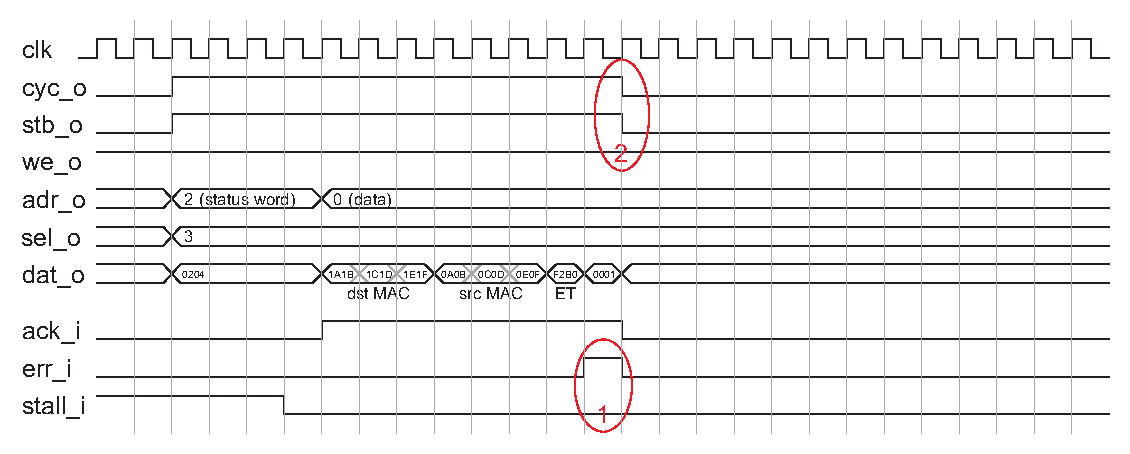
\includegraphics[width=\textwidth]{fig/basic_wrf_cycle_err.pdf}
    \caption{WR Fabric cycle interrupted with an error line}
    \label{fig:fabric:cycerr}
  \end{center}
\end{figure}

\begin{enumerate}
  \item WRF Sink wants to break a bus cycle, so it drives \emph{err\_i} high.
  \item WRF Source breaks the cycle immediately after receiving an error indicator
    from the WRF Sink.
\end{enumerate}

\newparagraph{SystemVerilog model}
The SystemVerilog simulation model of the WR Fabric interface (both WRF Source and 
WRF Sink) can be found in the \emph{wr-cores} git repository
(git://ohwr.org/hdl-core-lib/wr-cores.git) and consists of the files:
\begin{itemize}
  \item \emph{sim/if\_wb\_master.svh}
  \item \emph{sim/if\_wb\_slave.svh}
  \item \emph{sim/wb\_packet\_source.svh}
  \item \emph{sim/wb\_packet\_sink.svh}
\end{itemize}

The testbench example using the simulation model of WR Fabric interface can
be found in the zip archive attached to this documentation.


\subsubsection{Tx Timestamping interface}
\label{sec:txts}

The Tx Timestamping interface provides the timestamps generated inside WRPC for each
Ethernet frame transmitted from user-defined module through the WRF Sink interface.\\


\subsection{Aux clocks}

\begin{figure}[ht]
  \begin{center}
    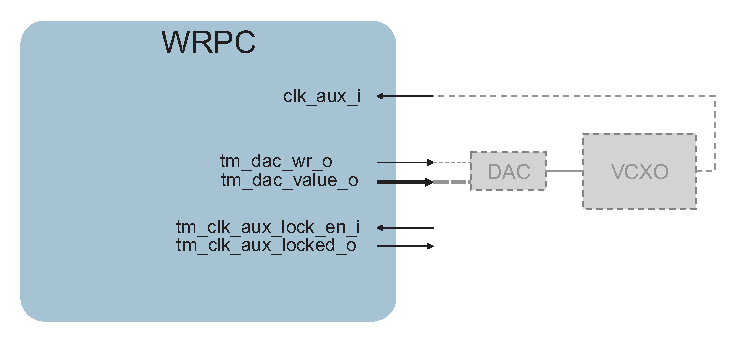
\includegraphics[width=.8\textwidth]{fig/adv_wrpc_clk.pdf}
    \caption{Aux clock synchronization interface}
  \end{center}
\end{figure}

The WRPC can syntonize auxiliary clock signals to the White Rabbit timebase. It
is done with a similar PLL that is used to discipline the local reference clock
(section \ref{basic:clk_rst}). WRPC provides tuning values for the VCXO producing
clock signal which is connected to \emph{clk\_aux\_i}.

\begin{hdlporttable}
\end{hdlporttable}

\subsubsection{Timecode interface}
\label{sec:wrpc_timecode}

%\begin{figure}[ht]
%  \begin{center}
%    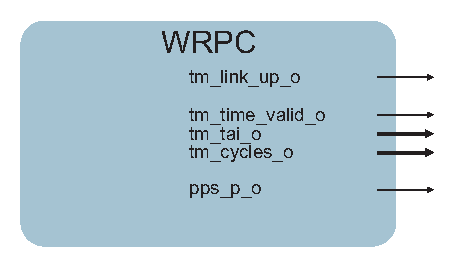
\includegraphics[width=.5\textwidth]{fig/basic_wrpc_tm.pdf}
%    \caption{Timecode output interface of WRPC}
%  \end{center}
%\end{figure}

Timecode interface provides current time to the other HDL modules in a form that
can be easily used. It consists of: a 1-PPS and a UTC timecode
aligned to the time of WR Master.


\subsection{Auxiliary diagnostics interface}
\label{sec:aux_diag}

Auxiliary diagnostics interface can be used if a user would like to benefit from
the WR PTP Core diagnostics capabilities to export some registers from his/her
IP core. The interface consists of two 32-bit \texttt{std\_logic\_vector}
arrays. User-defined registers that are to be read from the WRPC SNMP agent (SNMP
GET requests), should be connected to the \texttt{aux\_diag\_i} vector.
User-defined values that are written from the WRPC SNMP agent (SNMP SET
requests) will be available in the \texttt{aux\_diag\_o} vector.

Two VHDL generics \texttt{g\_diag\_id} and \texttt{g\_diag\_ver} are used to let
the user uniquely identify given application (user-defined set of registers)
to match it with appropriate, custom SNMP MIB file.


\subsection{Platform Support Packages}
\label{sec:hdl_platform}

The White Rabbit (WR) PTP core project provides platform support packages (PSPs) for Altera and
Xilinx FPGAs.

By using these modules, users gain the benefit of instantiating all the platform-specific support
components for the WR PTP core (PHY, PLLs, etc.) in one go, without having to delve into the
implementation details, using a setup that has been tested and is known to work well on the
supported FPGAs.

\subsubsection{Common}
\label{sec:hdl_platform_common}

This section describes the generic parameters and ports which are common to all provided PSPs.

\newparagraph{Generic parameters}

\begin{hdlparamtable}
  g\_with\_external\_clock\_input & boolean & false & Select whether to
  include the external 10MHz reference clock input (used in WR Grandmaster mode)\\
  \hline
  g\_use\_default\_plls & boolean & true & Set to FALSE if you want to
  instantiate your own PLLs\\
\end{hdlparamtable}

Each PSP provides two generic parameters of boolean type , which allow the users to configure the
PLLs in their designs. As such, four different PLL setups can be achieved by changing the values of
these parameters.

\begin{description}
\item[PLL setup 1:] Use default PLLs, no external reference clock. In this setup, the PSP expects
  one 20MHz and one 125MHz clock, and it will instantiate all the required PLLs internally. This is
  the default mode.
\item[PLL setup 2:] Use default PLLs, with external reference clock. This is the same as PLL setup
  1, with the addition of the external 10MHz reference clock input, which will be multiplied
  internally by the PSP to 125MHz.
\item[PLL setup 3:] Use custom PLLs, no external reference clock. In this setup, the PSP will not
  instantiate any PLLs internally. It is up to the user to provide the 62.5MHz system clock, the
  125MHz reference clock and the 62.5MHz DMTD clock.
\item[PLL setup 4:] Use custom PLLs, with external reference clock. This is the same as PLL setup 3,
  with the addition of the external reference clock input, which should be provided as is (10MHz)
  and also multiplied to 125MHz.
\end{description}

\newparagraph{Ports}

\begin{hdlporttable}
  areset\_n\_i & in & 1 & asynchronous reset (active low)\\
  \hline
  clk\_10m\_ext\_i & in & 1 & 10MHz external reference clock input
  (used when \tts{g\_with\_external\_clock\_input = true})\\
  \hline\pagebreak
  \hdltablesection{Clock inputs for default PLLs (used when
    \tts{g\_use\_default\_plls = true})}\\
  \hline
  clk\_20m\_vcxo\_i & in & 1 & 20MHz VCXO clock\\
  \hline
  clk\_125m\_pllref\_i & in & 1 & 125MHz PLL reference\\
  \hline
  \hdltablesection{Interface with custom PLLs (used when
    \tts{g\_use\_default\_plls = false})}\\
  \hline
  clk\_62m5\_dmtd\_i & in & 1 &  \multirowpar{2}{62.5MHz DMTD offset
    clock and lock status}\\
  \cline{1-3}
  clk\_dmtd\_locked\_i & in & 1 & \\
  \hline
  clk\_62m5\_sys\_i & in & 1 & \multirowpar{2}{62.5MHz Main system
    clock and lock status}\\
  \cline{1-3}
  clk\_sys\_locked\_i & in & 1 & \\
  \hline
  clk\_125m\_ref\_i & in & 1 & 125MHz Reference clock\\
  \hline
  clk\_125m\_ext\_i & in & 1 & \multirowpar{4}{125MHz derived
      from 10MHz external reference, locked/stopped status inputs and reset output (used when
      \tts{g\_with\_external\_clock\_input = true})}\\
  \cline{1-3}
  clk\_ext\_locked\_i & in & 1 & \\
  \cline{1-3}
  clk\_ext\_stopped\_i & in & 1 & \\
  \cline{1-3}
  clk\_ext\_rst\_o & out & 1 &\\
  \hline
  \hdltablesection{Interface with SFP}\\
  \hline
  sfp\_tx\_fault\_i & in & 1 & TX fault indicator\\
  \hline
  sfp\_los\_i & in & 1 & Loss Of Signal indicator\\
  \hline
  sfp\_tx\_disable\_o & out & 1 & TX disable control\\
  \hline
  \hdltablesection{Interface with WRPC}\\
  \hline
  clk\_62m5\_sys\_o & out & 1 & 62.5MHz system clock output\\
  \hline
  clk\_125m\_ref\_o & out & 1 & 125MHz reference clock output\\
  \hline
  clk\_62m5\_dmtd\_o & out & 1 & 62.5MHz DMTD clock output\\
  \hline
  pll\_locked\_o & out & 1 & logic AND of system and DMTD PLL lock\\
  \hline
  clk\_10m\_ext\_o & out & 1 & 10MHz external reference clock output\\
  \hline
  phy8\_o & out & rec & \multirowpar{2}{input/output records for PHY signals
    when \tts{g\_pcs\_16bit = false}}\\
  \cline{1-3}
  phy8\_i & in & rec & \\
  \hline
  phy16\_o & out & rec & \multirowpar{2}{input/output records for PHY signals
    when \tts{g\_pcs\_16bit = true}}\\
  \cline{1-3}
  phy16\_i & in & rec & \\
  \hline
  ext\_ref\_mul\_o & out & 1 & \multirowpar{4}{125MHz derived from
    10MHz external reference, locked/stopped status outputs and reset input}\\
  \cline{1-3}
  ext\_ref\_mul\_locked\_o & out & 1 & \\
  \cline{1-3}
  ext\_ref\_mul\_stopped\_o & out & 1 & \\
  \cline{1-3}
  ext\_ref\_rst\_i & in & 1 & \\
\end{hdlporttable}

\subsubsection{Altera}
\label{sec:hdl_platform_altera}

The Altera PSP currently supports the Arria V family of FPGAs.

The top-level VHDL module is located under:\\\hrefwrpc{platform/altera/xwrc\_platform\_altera.vhd}

A VHDL package with the definition of the module can be found
under:\\\hrefwrpc{platform/wr\_altera\_pkg.vhd}

An example (VHDL) instantiation of this module can be found in the VFC-HD board support package (see
also Section~\ref{sec:hdl_board_vfchd}):\\\hrefwrpc{board/vfchd/xwrc\_board\_vfchd.vhd}

This section describes the generic parameters and ports which are specific to the Altera
PSP. Parameters and ports common to all PSPs are described in Section~\ref{sec:hdl_platform_common}.

\newparagraph{Generic parameters}

\begin{hdlparamtable}
  g\_fpga\_family & string & arria5 & Defines the family/model of Altera
  FPGA. Recognized values are "arria5" (more will be added)\\
  \hline
  g\_pcs16\_bit & boolean & false & Some FPGA families provide the possibility
  to configure the PCS of the PHY as either 8bit or 16bit. The default is to use the 8bit PCS,
  but this generic can be used to override it\\
\end{hdlparamtable}

\newparagraph{Ports}

\begin{hdlporttable}
  \hdltablesection{Interface with SFP}\\
  \hline
  \linebreak sfp\_tx\_o\linebreak & out & 1 & \multirowpar{2}{PHY TX and RX. These
    are single ended and should be mapped to the positive half of each differential signal.
    Altera tools will infer both the negative half and the differential receiver}\\
  \cline{1-3}
  \linebreak sfp\_rx\_i\linebreak & in & 1 &\\
\end{hdlporttable}

\subsubsection{Xilinx}
\label{sec:hdl_platform_xilinx}

The Xilinx PSP currently supports the Spartan 6 family of FPGAs.

The top-level VHDL module is located under:\\ \hrefwrpc{platform/xilinx/xwrc\_platform\_xilinx.vhd}

A VHDL package with the definition of the module can be found
under:\\ \hrefwrpc{platform/wr\_xilinx\_pkg.vhd}

Examples of (VHDL) instantiation of this module can be found in the SPEC and SVEC board support
packages (see also Sections~\ref{sec:hdl_board_spec}
and~\ref{sec:hdl_board_svec}):\\
\hrefwrpc{board/spec/xwrc\_board\_spec.vhd}\\
\hrefwrpc{board/svec/xwrc\_board\_svec.vhd}

This section describes the generic parameters and ports which are
specific to the Xilinx PSP. Parameters and ports common to all PSPs
are described in Section~\ref{sec:hdl_platform_common}.

\newparagraph{Generic parameters}

\begin{hdlparamtable}
  g\_fpga\_family & string & spartan6 & Defines the family/model of Xilinx
  FPGA. Recognized values are "spartan6" (more will be added)\\
  \hline
  g\_simulation & integer & 0 & setting to '1' speeds up the simulation, must
  be set to '0' for synthesis\\
\end{hdlparamtable}

\newparagraph{Ports}

\begin{hdlporttable}
  clk\_125m\_gtp\_p\_i & in & 1 & \multirowpar{2}{125MHz GTP
    reference differential clock input}\\
  \cline{1-3}
  clk\_125m\_gtp\_n\_i & in & 1 & \\
  \hline
  \hdltablesection{Interface with SFP}\\
  \hline
  sfp\_txn\_o & out & 1 & \multirowpar{2}{differential pair for PHY TX}\\
  \cline{1-3}
  sfp\_txp\_o & out & 1 & \\
  \hline
  sfp\_rxn\_i & in & 1 & \multirowpar{2}{differential pair for PHY RX}\\
  \cline{1-3}
  sfp\_rxp\_i & in & 1 & \\
\end{hdlporttable}

\section{Board Support Packages}
\label{sec:hdl_board}

The White Rabbit (WR) PTP core project provides board support packages (BSPs) for the following
boards:
\begin{itemize}
\item \href{http://www.ohwr.org/projects/spec}{SPEC}, a PCIe single FMC carrier board based on a
  Xilinx Spartan 6 FPGA.
\item \href{http://www.ohwr.org/projects/svec}{SVEC}, a VME dual FMC carrier board based on a Xilinx
  Spartan 6 FPGA.
\item \href{http://www.ohwr.org/projects/vfc-hd}{VFC-HD}, a VME single FMC carrier board based on an
  Altera Arria V FPGA.
\end{itemize}

By using these modules, users gain the benefit of instantiating all the necessary components of the
WR PTP core (including the core itself, the PHY, PLLs, etc.) in one go, without having to delve into
the implementation details, using a setup that has been tested and is known to work well on the
supported boards.

Each BSP is split in two modules: the common module, which is shared across all BSPs, and the
board-specific module. The common module instantiates the WRPC itself, together with a selection of
interfaces for connecting the core the the user FPGA logic. The board-specific module instantiates
all the FPGA- and system-specific parts (related to WR), such as hard IP provided by the FPGA
vendor, interfaces to DACs, reset inputs, etc.

The BSPs make use internally of the appropriate FPGA family platform support packages (PSPs, see also
Section~\ref{sec:hdl_platform}). For users who need more control and flexibility over their designs,
it is suggested to use the BSP as a reference, and to consider instantiating directly the respective
PSP for their FPGA family.

\subsection{Common}
\label{sec:hdl_board_common}

Most of the generic parameters and ports of the board-common module map directly to those of the
WRPC. One notable exception to this rule is that of the parameters and ports related to the selected
interface for connecting the core to the user FPGA logic.

The board-common module provides the \tts{g\_fabric\_iface} generic parameter, an enumeration
type with three possible values:

\begin{description}
\item[PLAIN:] No additional module is instantiated and the ``raw'' WRPC fabric interface (see also
  Section~\ref{sec:wrpc_fabric}) is provided on the board's ports.
\item[STREAMERS:] A set of \href{http://www.ohwr.org/projects/wr-cores/wiki/WR_Streamers}{TX/RX
  streamers} is attached to the WRPC fabric interface.
\item[ETHERBONE:] An \href{http://www.ohwr.org/projects/etherbone-core/wiki}{Etherbone} slave node
  is attached to the WRPC fabric interface.
\end{description}

Sections~\ref{sec:hdl_board_common_param} and~\ref{sec:hdl_board_common_ports} list the generic
parameters and ports of the board-common module which are shared across the BSPs.

\textbf{Note:} the board-common module defines more parameters and ports than the ones mentioned in
the following sections. Those that are not exposed by any of the BSPs have been left out to keep the
tables short and to the point. Users interested in studying the board-common module and/or writing
their own BSP, can find the board-common module under:
\\\hrefwrpc{board/common/xwrc\_board\_common.vhd}

\subsubsection{Generic parameters}
\label{sec:hdl_board_common_param}

\begin{hdlparamtable}
  g\_simulation & integer & 0 & \multirowpar{11}{These map directly to generic parameters with the
    same name in the WRPC module (see Section~\ref{sec:wrc_generics})}\\
  \cline{1-3}
  g\_with\_external\_clock\_input & boolean & true & \\
  \cline{1-3}
  g\_aux\_clks & integer & 0 & \\
  \cline{1-3}
  g\_dpram\_initf & string & "" & \\
  \cline{1-3}
  g\_diag\_id & integer & 0 & \\
  \cline{1-3}
  g\_diag\_ver & integer & 0 & \\
  \cline{1-3}
  g\_diag\_ro\_size & integer & 0 & \\
  \cline{1-3}
  g\_diag\_rw\_size & integer & 0 & \\
  \hline
  g\_tx\_streamer\_width & integer & 32 & \multirowpar{2}{TX/RX
    data width when \tts{g\_fabric\_iface = STREAMERS} (otherwise ignored)}\\
  \cline{1-3}
  g\_rx\_streamer\_width & integer & 32 & \\
  \hline
  g\_fabric\_iface & enum & PLAIN & optional module to be attached to the
  fabric interface of WRPC \tts{[PLAIN/STREAMERS/ETHERBONE]}\\
\end{hdlparamtable}

\subsubsection{Ports}
\label{sec:hdl_board_common_ports}

\begin{hdlporttable}
  \hdltablesection{Clocks and resets}\\
  \hline
  clk\_aux\_i & in & var & [optional] vector of auxiliary
  clocks that will be disciplined to WR timebase. Size is equal to \tts{g\_aux\_clks}\\
  \hline
  clk\_ext\_i & in & 1 & 10MHz external reference clock input
  (used when \tts{g\_with\_external\_clock\_input = true})\\
  \hline
  pps\_ext\_i & in & 1 & external 1-PPS input (used when
  \tts{g\_with\_external\_clock\_input = true})\\
  \hline
  clk\_sys\_62m5\_o & out & 1 & 62.5MHz system clock output\\
  \hline
  clk\_ref\_125m\_o & out & 1 & 125MHz reference clock output\\
  \hline
  rst\_62m5\_n\_o & out & 1 & Active low reset output, synchronous to \tts{clk\_sys\_62m5\_o}\\
  \hline
  rst\_125m\_n\_o & out & 1 & Active low reset output, synchronous to \tts{clk\_ref\_125m\_o}\\
  \hline
  \hdltablesection{Interface with SFP}\\
  \hline
  sfp\_tx\_fault\_i & in & 1 & TX fault indicator\\
  \hline
  sfp\_los\_i & in & 1 & Loss Of Signal indicator\\
  \hline
  sfp\_tx\_disable\_o & out & 1 & TX disable control\\
  \hline
  \hdltablesection{I2C EEPROM interface}\\
  \hline
  eeprom\_sda\_i & in  & 1 & \multirowpar{2}{EEPROM I2C SDA}\\
  \cline{1-3}
  eeprom\_sda\_o & out & 1 & \\
  \hline
  eeprom\_scl\_i & in  & 1 & \multirowpar{2}{EEPROM I2C SCL}\\
  \cline{1-3}
  eeprom\_scl\_o & out & 1 & \\
  \hline
  \hdltablesection{Onewire interface (UID and temperature)}\\
  \hline
  onewire\_i & in  & 1 & OneWire data input\\
  \hline
  onewire\_oen\_o & out & 1 & OneWire data output enable (when asserted,
  OneWire tri-state output buffer should be enabled and driven to ground)\\
  \hline
  \hdltablesection{External WishBone interface}\\
  \hline
  wb\_slave\_o & out & rec & \multirowpar{2}{Mapped to WRPC external WB slave
    interface (see also Section~\ref{sec:wrpc_wb})}\\
  \cline{1-3}
  wb\_slave\_i & in & rec & \\
  \hline
  \hdltablesection{WR fabric interface (when \tts{g\_fabric\_iface = plain})}\\
  \hline
  wrf\_src\_o & out & rec & \multirowpar{4}{Mapped to WRPC fabric interface
    (see also Section~\ref{sec:wrpc_fabric})}\\
  \cline{1-3}
  wrf\_src\_i & in &  rec & \\
  \cline{1-3}
  wrf\_snk\_o & out & rec & \\
  \cline{1-3}
  wrf\_snk\_i & in &  rec & \\
  \hline
  \hdltablesection{WR streamers (when \tts{g\_fabric\_iface = streamers})}\\
  \hline
  wrs\_tx\_data\_i & in &  var & Data to be sent. Size is equal to \tts{g\_tx\_streamer\_width}\\
  \hline
  wrs\_tx\_valid\_i & in & 1 & Indicates whether \tts{wrs\_tx\_data\_i} contains valid data\\
  \hline
  wrs\_tx\_dreq\_o & out & 1 & When active, the user may send a data word in the
  following clock cycle\\
  \hline
  wrs\_tx\_last\_i & in &  1 & Can be used to indicate the last data word in a
  larger block of samples\\
  \hline
  wrs\_tx\_flush\_i & in &  1 & When asserted, the streamer will immediatly send
  out all the data that is stored in its TX buffer\\
  \hline
  wrs\_rx\_first\_o & out & 1 & Indicates the first word of the data block on \tts{wrs\_rx\_data\_o}\\
  \hline
  wrs\_rx\_last\_o & out & 1 & Indicates the last word of the data block on \tts{wrs\_rx\_data\_o}\\
  \hline
  wrs\_rx\_data\_o & out & var & Received data. Size is equal to \tts{g\_rx\_streamer\_width}\\
  \hline
  wrs\_rx\_valid\_o & out & 1 & Indicates that \tts{wrs\_rx\_data\_o} contains valid data\\
  \hline
  wrs\_rx\_dreq\_i & in &  1 & When asserted, the streamer may output another data word in the
  subsequent clock cycle\\
  \hline
  \hdltablesection{Etherbone WB master interface (when \tts{g\_fabric\_iface = etherbone})}\\
  \hline
  \linebreak wb\_eth\_master\_o\linebreak & out & rec & \multirowpar{2}{WB master interface for the
    Etherbone core. Normally this is attached to a slave port of the primary WB crossbar in the design,
    in order to provide access to all WB peripherals over Etherbone}\\
  \cline{1-3}
  \linebreak wb\_eth\_master\_i\linebreak & in & rec & \\
  \hline
  \hdltablesection{Generic diagnostics interface}\\
  \hline
  \linebreak aux\_diag\_i\linebreak & in & var & \multirowpar{2}{Arrays of 32~bit vectors, to be
    accessed from WRPC via SNMP or uart console. Input array contains \tts{g\_diag\_ro\_size},
    while output array contains \tts{g\_diag\_rw\_size} elements.}\\
  \cline{1-3}
  \linebreak aux\_diag\_o\linebreak & out & var & \\
  \hline
  \hdltablesection{Auxiliary clocks control}\\
  \hline
  tm\_dac\_value\_o & out & 24 & DAC value for tuning auxiliary clock
  (\emph{clk\_aux\_i})\\
  \hline
  tm\_dac\_wr\_o & out & var & validates auxiliary DAC value. Size is equal
  to \tts{g\_aux\_clks}\\
  \hline
  tm\_clk\_aux\_lock\_en\_i & in & var & enable locking auxiliary clock to
  internal WR clock. Size is equal to \tts{g\_aux\_clks}\\
  \hline
  tm\_clk\_aux\_locked\_o & out & var & auxiliary clock locked to internal WR
  clock. Size is equal to \tts{g\_aux\_clks}\\
  \hline  
  \hdltablesection{External TX timestamp interface}\\
  \hline
  timestamps\_o & out & rec & Record-based output ports for
  the TX timestamp interface (see also Section~\ref{sec:txts})\\
  \hline
  txtsu\_ack\_i & in & 1 & acknowledge, indicating that user-defined module
  has received the timestamp\\
  \hline 
  \hdltablesection{Pause frame control}\\
  \hline
  fc\_tx\_pause\_req\_i   & in  &  1 & \\
  \hline
  fc\_tx\_pause\_delay\_i & in  & 16 & \\
  \hline
  fc\_tx\_pause\_ready\_o & out &  1 & \\
  \hline
  \hdltablesection{WRPC timecode interface}\\
  \hline
  tm\_link\_up\_o & out & 1 & state of Ethernet link (up/down), \emph{1}
  means Ethernet link is up\\
  \hline
  tm\_time\_valid\_o & out & 1 & if \emph{1}, the timecode generated by the
  WRPC is valid\\
  \hline
  tm\_tai\_o & out & 40 & TAI part of the timecode (full seconds)\\
  \hline
  tm\_cycles\_o & out & 28 & fractional part of each second represented by
  the state of counter clocked with the frequency 125 MHz (values from 0 to
  124999999, each count is 8 ns)\\
  \hline
  \hdltablesection{Buttons, LEDs and PPS output}\\
  \hline
  led\_act\_o & out & 1 & signal for driving Ethernet activity LED\\
  \hline
  led\_link\_o & out & 1 & signal for driving Ethernet link LED\\
  \hline
  btn1\_i & in & 1 & \multirowpar{2}{two microswitch inputs, active low, currently not
    used in official WRPC software}\\
  \cline{1-3}
  btn2\_i & in & 1 & \\
  \hline
  pps\_p\_o & out & 1 & 1-PPS signal generated in \tts{clk\_ref\_i} clock
  domain and aligned to WR time, pulse generated when the cycle counter is 0
  (beginning of each full TAI second)\\
  \hline
  pps\_led\_o & out & 1 & 1-PPS signal with extended pulse width to drive a LED\\
  \hline
  link\_ok\_o & out & 1 & Link status indicator\\
\end{hdlporttable}

\subsection{SPEC}
\label{sec:hdl_board_spec}

The SPEC BSP provides a ready-to-use WRPC wrapper for the
\href{http://www.ohwr.org/projects/spec}{SPEC carrier board}.

The top-level VHDL module is located under: \\\hrefwrpc{board/spec/xwrc\_board\_spec.vhd}

An alternative top-level VHDL module which only makes use of standard logic for ports and integers
and strings for generic parameters (ideal for instantiation in Verilog-based designs) can be found
under: \\\hrefwrpc{board/spec/wrc\_board\_spec.vhd}

A VHDL package with the definition of both modules can be found under:
\\\hrefwrpc{board/spec/wr\_spec\_pkg.vhd}

An example (VHDL) instantiation of this module can be found in the SPEC WRPC reference design:
\\\hrefwrpc{top/spec\_ref\_design/spec\_wr\_ref\_top.vhd}

This section describes the generic parameters and ports which are specific to the SPEC BSP.
Parameters and ports common to all BSPs are described in Section~\ref{sec:hdl_board_common}.

\subsubsection{Generic parameters}

No additional generic parameters are declared in the SPEC BSP. See
Section~\ref{sec:hdl_board_common_param} for a the list of common BSP parameters.


\subsubsection{Ports}

\begin{hdlporttable}
  \hdltablesection{Clocks and resets}\\
  \hline
  areset\_n\_i & in & 1 & Reset input (active low, can be async)\\
  \hline
  clk\_20m\_vcxo\_i & in & 1 & 20MHz clock input from board VCXO\\
  \hline
  clk\_125m\_pllref\_p\_i & in & 1 & \multirowpar{2}{125MHz PLL reference
    differential clock input from board}\\
  \cline{1-3}
  clk\_125m\_pllref\_n\_i & in & 1 & \\
  \hline
  clk\_125m\_gtp\_p\_i & in & 1 & \multirowpar{2}{125MHz GTP
    reference differential clock input from board}\\
  \cline{1-3}
  clk\_125m\_gtp\_n\_i & in & 1 & \\
  \hline
  \hdltablesection{SPI interface to DACs}\\
  \hline
  plldac\_sclk\_o & out & 1 & SPI SCLK, common to both DACs\\
  \hline
  plldac\_din\_o & out & 1 & SPI MOSI, common to both DACs\\
  \hline
  pll25dac\_cs\_n\_o & out & 1 & SPI $\overline{\mbox{SS}}$ for DAC controlling 25MHz oscillator\\
  \hline
  pll20dac\_cs\_n\_o & out & 1 & SPI $\overline{\mbox{SS}}$ for DAC controlling 20MHz oscillator\\
  \hline
  \hdltablesection{SFP interface}\\
  \hline
  sfp\_txn\_o & out & 1 & \multirowpar{2}{differential pair for PHY TX}\\
  \cline{1-3}
  sfp\_txp\_o & out & 1 & \\
  \hline
  sfp\_rxn\_i & in & 1 & \multirowpar{2}{differential pair for PHY RX}\\
  \cline{1-3}
  sfp\_rxp\_i & in & 1 & \\
  \hline
  sfp\_det\_i & in  & 1 & Active low, indicates presence of SFP (corresponds to SFP MOD-DEF0)\\
  \hline
  sfp\_sda\_i & in  & 1 & \multirowpar{2}{SFP I2C SDA}\\
  \cline{1-3}
  sfp\_sda\_o & out & 1 & \\
  \hline
  sfp\_scl\_i & in  & 1 & \multirowpar{2}{SFP I2C SCL}\\
  \cline{1-3}
  sfp\_scl\_o & out & 1 & \\
  \hline
  sfp\_rate\_select\_o & out & 1 & SFP rate select\\
  \hline
  \hdltablesection{Physical UART interface}\\
  \hline
  uart\_rxd\_i & in  & 1 & UART RXD (serial data to WRPC)\\
  \hline
  uart\_txd\_o & out & 1 & UART TXD (serial data from WRPC)\\
  \hline
  \hdltablesection{Flash memory SPI interface}\\
  \hline
  flash\_sclk\_o & out & 1 & Flash SPI SCLK\\
  \hline
  flash\_ncs\_o  & out & 1 & Flash SPI $\overline{\mbox{SS}}$\\
  \hline
  flash\_mosi\_o & out & 1 & Flash SPI MOSI\\
  \hline
  flash\_miso\_i & in  & 1 & Flash SPI MISO\\
\end{hdlporttable}

\subsection{SVEC}
\label{sec:hdl_board_svec}

The SVEC BSP provides a ready-to-use WRPC wrapper for the
\href{http://www.ohwr.org/projects/svec}{SVEC carrier board}.

The top-level VHDL module is located under: \\\hrefwrpc{board/svec/xwrc\_board\_svec.vhd}

An alternative top-level VHDL module which only makes use of standard logic for ports and integers
and strings for generic parameters (ideal for instantiation in Verilog-based designs) can be found
under: \\\hrefwrpc{board/svec/wrc\_board\_svec.vhd}

A VHDL package with the definition of both modules can be found under:
\\\hrefwrpc{board/svec/wr\_svec\_pkg.vhd}

An example (VHDL) instantiation of this module can be found in the SVEC WRPC reference design:
\\\hrefwrpc{top/svec\_ref\_design/svec\_wr\_ref\_top.vhd}

This section describes the generic parameters and ports which are specific to the SVEC BSP.
Parameters and ports common to all BSPs are described in Section~\ref{sec:hdl_board_common}.

\subsubsection{Generic parameters}

No additional generic parameters are declared in the SVEC BSP. See
Section~\ref{sec:hdl_board_common_param} for a the list of common BSP parameters.

\subsubsection{Ports}

\begin{hdlporttable}
  \hdltablesection{Clocks and resets}\\
  \hline
  areset\_n\_i & in & 1 & Reset input (active low, can be async)\\
  \hline
  clk\_20m\_vcxo\_i & in & 1 & 20MHz clock input from board VCXO\\
  \hline
  clk\_125m\_pllref\_p\_i & in & 1 & \multirowpar{2}{125MHz PLL reference
    differential clock input from board}\\
  \cline{1-3}
  clk\_125m\_pllref\_n\_i & in & 1 & \\
  \hline
  clk\_125m\_gtp\_p\_i & in & 1 & \multirowpar{2}{125MHz GTP
    reference differential clock input from board}\\
  \cline{1-3}
  clk\_125m\_gtp\_n\_i & in & 1 & \\
  \hline
  \hdltablesection{SPI interface to DACs}\\
  \hline
  pll20dac\_sclk\_o & out & 1 & SPI SCLKfor DAC controlling 20MHz oscillator\\
  \hline
  pll20dac\_din\_o & out & 1 & SPI MOSI for DAC controlling 20MHz oscillator\\
  \hline
  pll20dac\_cs\_n\_o & out & 1 & SPI $\overline{\mbox{SS}}$ for DAC controlling 20MHz oscillator\\
  \hline
  pll25dac\_sclk\_o & out & 1 & SPI SCLK for DAC controlling 25MHz oscillator\\
  \hline
  pll25dac\_din\_o & out & 1 & SPI MOSI for DAC controlling 25MHz oscillator\\
  \hline
  pll25dac\_cs\_n\_o & out & 1 & SPI $\overline{\mbox{SS}}$ for DAC controlling 25MHz oscillator\\
  \hline
  \hdltablesection{SFP interface}\\
  \hline
  sfp\_txn\_o & out & 1 & \multirowpar{2}{differential pair for PHY TX}\\
  \cline{1-3}
  sfp\_txp\_o & out & 1 & \\
  \hline
  sfp\_rxn\_i & in & 1 & \multirowpar{2}{differential pair for PHY RX}\\
  \cline{1-3}
  sfp\_rxp\_i & in & 1 & \\
  \hline
  sfp\_det\_i & in  & 1 & Active low, indicates presence of SFP (corresponds to SFP MOD-DEF0)\\
  \hline
  sfp\_sda\_i & in  & 1 & \multirowpar{2}{SFP I2C SDA}\\
  \cline{1-3}
  sfp\_sda\_o & out & 1 & \\
  \hline
  sfp\_scl\_i & in  & 1 & \multirowpar{2}{SFP I2C SCL}\\
  \cline{1-3}
  sfp\_scl\_o & out & 1 & \\
  \hline
  sfp\_rate\_select\_o & out & 1 & SFP rate select\\
  \hline
  \hdltablesection{Physical UART interface}\\
  \hline
  uart\_rxd\_i & in  & 1 & UART RXD (serial data to WRPC)\\
  \hline
  uart\_txd\_o & out & 1 & UART TXD (serial data from WRPC)\\
  \hline
  \hdltablesection{Flash memory SPI interface}\\
  \hline
  spi\_sclk\_o & out & 1 & Flash SPI SCLK\\
  \hline
  spi\_ncs\_o  & out & 1 & Flash SPI $\overline{\mbox{SS}}$\\
  \hline
  spi\_mosi\_o & out & 1 & Flash SPI MOSI\\
  \hline
  spi\_miso\_i & in  & 1 & Flash SPI MISO\\
\end{hdlporttable}

\subsection{VFC-HD}
\label{sec:hdl_board_vfchd}

The VFC-HD BSP provides a ready-to-use WRPC wrapper for the
\href{http://www.ohwr.org/projects/vfc-hd}{VFC-HD carrier board}.

The top-level VHDL module is located under: \\\hrefwrpc{board/vfchd/xwrc\_board\_vfchd.vhd}

An alternative top-level VHDL module which only makes use of standard logic for ports and integers
and strings for generic parameters (ideal for instantiation in Verilog-based designs) can be found
under: \\\hrefwrpc{board/vfchd/wrc\_board\_vfchd.vhd}

A VHDL package with the definition of both modules can be found under:
\\\hrefwrpc{board/vfchd/wr\_vfchd\_pkg.vhd}

An example (VHDL) instantiation of this module can be found in the VFC-HD WRPC reference design:
\\\hrefwrpc{top/vfchd\_ref\_design/vfchd\_wr\_ref\_top.vhd}

This section describes the generic parameters and ports which are specific to the VFC-HD BSP.
Parameters and ports common to all BSPs are described in Section~\ref{sec:hdl_board_common}.

\subsubsection{Generic parameters}

\begin{hdlparamtable}
  g\_pcs16\_bit & boolean & false & Altera Arria V FPGAs provide the possibility
  to configure the PCS of the PHY as either 8bit or 16bit. The default is to use the 8bit PCS,
  but this generic can be used to override it\\
\end{hdlparamtable}

\subsubsection{Ports}

\begin{hdlporttable}
  \hdltablesection{Clocks and resets}\\
  \hline
  areset\_n\_i & in & 1 & Reset input (active low, can be async)\\
  \hline
  clk\_board\_20m\_i & in & 1 & 20MHz clock input from board\\
  \hline
  clk\_board\_125m\_i & in & 1 & 125MHz reference clock input from board\\
  \hline
  \hdltablesection{SPI interface to DACs}\\
  \hline
  dac\_sclk\_o & out & 1 & SPI SCLK, common to both DACs\\
  \hline
  dac\_din\_o & out & 1 & SPI MOSI, common to both DACs\\
  \hline
  dac\_ref\_sync\_n\_o & out & 1 & SPI $\overline{\mbox{SS}}$ for DAC controlling 125MHz oscillator\\
  \hline
  dac\_dmtd\_sync\_n\_o & out & 1 & SPI $\overline{\mbox{SS}}$ for DAC controlling 20MHz oscillator\\
  \hline
  \hdltablesection{SFP interface}\\
  \hline
  sfp\_tx\_o & out & 1 & PHY TX\\
  \hline
  sfp\_rx\_i & in & 1 & PHY RX\\
  \hline
  sfp\_det\_i & in  & 1 & Active high, asserted if all of the following are true:\linebreak
  * SFP is detected (plugged in)\linebreak
  * The part number has been successfully read\\
  \hline
  sfp\_data\_i & in  & 128 & 16 byte SFP vendor Part Number (ASCII encoded, first character byte
  in bits 127 downto 120)\\

\end{hdlporttable}


\appendix
\bibliographystyle{unsrt}
\bibliography{references}

\end{document}
